\chapter{Il livello dei processi}

\section{Scheduling a basso livello}

Lo \textit{scheduling a basso livello} è il complesso di funzionalità per la gestione degli \textit{stati di avanzamento dei processi} e quindi la gestione della risorsa processore.

\begin{figure}[H]
    \centering
    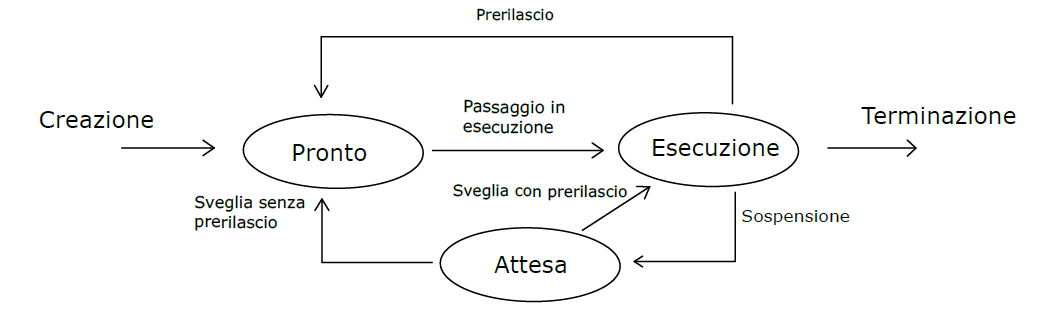
\includegraphics[width=\textwidth]{immagini/Scheduler.png}
\end{figure}

\noindent Nello stato di \textit{esecuzione} (``running'') un processo $Q$ utilizza effettivamente la risorsa processore per eseguire le proprie istruzioni.\
Nello stato di \textit{pronto} $Q$ ha tutte le caratteristiche per essere eseguibile, eccetto la disponibilità della risorsa processore; nel frattempo, in generale, esistono uno o più processi che precedono $Q$ in un ordinamento di processi pronti e quindi destinati a utilizzare il processore (Lista Pronti).\
Nello stato di \textit{attesa} $Q$ è sospeso nei confronti del verificarsi di un certo evento logico, senza dunque avere possibilità di essere eseguito, nemmeno se una risorsa processore fosse disponibile, fintanto che tale evento non si sarà verificato.

Il passaggio da \textit{esecuzione} ad \textit{attesa} provoca la conseguente \textit{commutazione di contesto} (del processore) per permettere il passaggio di un altro processo da \textit{pronto} a \textit{esecuzione}.

Quando si verifica l'evento sul quale un processo si è sospeso, il processo viene risvegliato e passa in stato di \textit{pronto}.

Se è prevista una priorità dei processi e il processo svegliato ha priorità più alta del processo in \textit{esecuzione}, si può avere la transizione da \textit{attesa} direttamente a \textit{esecuzione} con conseguente passaggio del processo ``running'' da \textit{esecuzione} a \textit{pronto} (\textit{prerilascio} del processore).

In generale, il \textit{prerilascio di un processore} si può verificare in due occasioni distinte:
\begin{enumerate}
    \item un processo A in \textit{attesa} viene svegliato da un processo B e A ha priorità maggiore di B: A passa direttamente in \textit{esecuzione} sul processore utilizzato da B, e B passa in stato di \textit{pronto};
    \item un processo A in \textit{esecuzione} passa in stato di \textit{pronto} per permettere al primo processo \textit{pronto} di passare in \textit{esecuzione}: questo meccanismo viene utilizzato nella gestione del processore \textit{a quanti di tempo}, in modo da bilanciare l'utilizzazione del processore stesso da parte di processi ``lunghi'', e/o con scarse occasioni di cooperazione con altri processi, e di processi ``corti'', e/o con frequenti
          interazioni con altri processi.
\end{enumerate}

\noindent Lo scheduling a quanti di tempo utilizza un'apposita unità di I/O che funge da \textit{Timer}; a distanza di un quanto di tempo (scandito da un certo numero di cicli di clock dell'unità), tale unità invia un'\textit{interruzione} di ``fine quanto di tempo'': il suo trattamento consiste nella \textit{sequenza di azioni per effettuare il prerilascio del processore}.

Una volta \textit{creato}, un processo passa in stato di \textit{pronto}.

Eseguendo l'istruzione \texttt{END} il processo \textit{termina}.

